\section{Approach}

We first describe stress test operators for evaluating robustness in
models, and adopt a subset of them as proxy test for short circuits. 
Then we modify some of these methods to create
training data to reverse the short circuit problem
and enhance the robustness of the models.
 \subsection{Stress Test Operators}
 \label{sec:stressop}
Short circuit behavior can be considered as a specific type of model fragility. The typical approach for detecting and evaluating model fragility is to construct stress test in addition to the original in-domain test set and observe model performance on these stress test.

In this paper , we consider the operators for constructing stress test listed in \tabref{table:proxyop}. Some of the operators were mentioned in previous literature, others are proposed here~(marked with *). Each operator creates stress test instance corresponding to a specific MCQ by keeping the right choice and generating a new \textbf{wrong} choice. The new wrong choice can be generated from 
three sources depending on the operator: a) right choice of the original MCQ; 
b) wrong choice of the original MCQ; c) right choice of another randomly 
sampled MCQ. 

While most of the operators are self-explanatory,
the \textit{crossover} operator is a little different and worth special mentioning.
This operator is inspired by molecular biology.
For each MCQ in the dataset that is correctly answered by the model, 
we substitute its original wrong choice with the right choice from 
another randomly sampled MCQ. The substituted choice in the new (proxy) 
question is guaranteed to be wrong. The operation can be visually
explained in \figref{fig:cross}. 

\begin{table}[th]
        \centering
        \scriptsize
        \begin{tabular}{l|l}
                \toprule
                \textbf{Oper.} &\textbf{Description and Example}\\
                \hline
                \multirow{3}{*}{Neg+} & Add negation (r$\rightarrow$w) \\
                & Input: \textit{They called the police to come to my house. \checksymbol} \\
                & Output: \textit{They {\color{olive}{didn't}}  called the police to come to my house. \crosssymbol} \\
                \hline
                \multirow{3}{*}{Neg-} &Remove negation (r$\rightarrow$w) \\
                & Input: \textit{Ben {\color{olive} never} starts working out. \checksymbol} \\
                & Output: \textit{Ben starts working out. \crosssymbol}\\
                \hline

                \multirow{3}{*}{NER} &Randomly replace person names (r$\rightarrow$w)\\
                 & Input: \textit{A big wave knocked {\color{olive} Mary} down . \checksymbol} \\
                & Output: \textit{A big wave knocked {\color{olive} Kia} down . \crosssymbol} \\
                \hline
                \multirow{3}{*}{PR*} & Switch pronoun by gender or quantity (r$\rightarrow$w)\\
        &Input: \textit{{\color{olive} She} had a great time .\checksymbol} \\
        &Output: \textit{{\color{olive} He} had a great time . \crosssymbol} \\
                \hline
                \multirow{3}{*}{PI*} &Instantiate pronoun by randome person (r$\rightarrow$w) \\
        &Input: \textit{{\color{olive} They} gave Tom a new latte with less ice . \checksymbol}\\
        &Output: \textit{{\color{olive} Nathanael} gave Tom a new latte with less ice . \crosssymbol}\\
                \bottomrule
%               \hline
                \multirow{3}{*}{Adv} &Add adverbs for emphasis (w$\rightarrow$w)\\
                &Input: \textit{The ocean was a calm as a bathtub .\crosssymbol} \\
                &Output: \textit{{\color{olive} In fact} the ocean was a calm as a bathtub .\crosssymbol} \\
                \hline
               \multirow{3}{*}{CO*} & Crossover: Swap the true choices between two questions (r$\rightarrow$w)\\ 
	&Input: \textit{\color{olive}Josh got sick . \checksymbol} \\
	&Output: \textit{\color{olive}{She had a great time .\crosssymbol}}  \\
\hline
                \multirow{3}{*}{Syn} &Replace adj/adv with synonym (w$\rightarrow$w) \\
                &Input: \textit{Dawn felt {\color{olive} happy} about getting away with it . \crosssymbol} \\
                &Output: \textit{Dawn felt {\color{olive} glad} about getting away with it . \crosssymbol} \\

		\bottomrule
               \multirow{3}{*}{MT*} & Mutate: Swap two consecutive words (r/w$\rightarrow$w) \\
		& Input: \textit{Deb said yes {\color{olive} to} {\color{olive} Tim} 's marriage proposal. \crosssymbol} \\
		& Output: \textit{Deb said yes {\color{olive} Tim} {\color{olive} to} 's marriage proposal .\crosssymbol} \\
		& Input: \textit{Josh {\color{olive}got sick}. \checksymbol} \\
		& Output: \textit{Josh {\color{olive} sick got}. \crosssymbol} \\
               \hline
\multirow{3}{*}{Voice} &Swap subject and object (r$\rightarrow$w) \\
        & Input: \textit{{\color{olive}{Kara}} asked {\color{olive}{the neighbors}}  not to litter in their yard . \checksymbol} \\
        & Output: \textit{{\color{olive}{the neighbors}} asked  {\color{olive}{Kara}}  not to litter in their yard . \crosssymbol}\\
                \bottomrule
        \end{tabular}
        \caption{Stress test operators considered in this paper. 
First line in each cell describes the operation, the remaining lines in
the cell give examples of how the operators work using input and output. 
r$\rightarrow$w indicates the operator turns a right choice into a wrong choice, while
w$\rightarrow$w indicates the operator turns a wrong choice into another wrong choice.} 
        \label{table:proxyop}
\end{table}

\subsection{Proxy Test for Short Circuit}
\label{sec:proxytest}
%\subsubsection*{Attention Score Analysis}
We propose a black-box framework to test short circuits in models. In a black-box testing, 
if a model correctly answers an MCQ, we create a new MCQ from
the old one by keeping the right choice of the old MCQ and 
generating a new wrong choice. The new wrong choice is generated by operations upon either the right choice of the old MCQ or the right choice of another randomly sampled MCQ.

%These operations can create additional questions from
%original ones to serve as stress test. We will discuss
%the suitability of these two operations for creating
%short-circuit tests. 
\cut{%%%%%%%%%%%%%%%%%%%%
\subsubsection*{White-box Attention Weights~(AW)}
%\KZ{Here we first talk about human testing by visualizastion,
%then talk about how to automatic it thru code.}

%show human annotation results of bert, roberta, xlnet.
One intuitive way to detect if an attention-based model is 
exploiting short circuits is to visualize its attention map. 
Given a well-trained model and a correctly answered MCQ  in the 
form of \textit{[CLS] premise [SEP] choice [SEP]}, 
where \textit{[CLS]} and \textit{[SEP]} are model-dependent 
delimiters and \textit{choice} refers to the right choice, 
we first tokenize the input, feed the token sequence into the model, 
and extract the attention map of all attention heads from the 
last encoder layer.

The attention maps are visualized through off-the-shelf tool~\cite{vig-2019-multiscale}
into user-friendly demo as shown in \figref{fig:att-goodex}. 
Human annotators are then asked to determine whether there exists 
strong attention connections from the right choice to the premise. 
We consider the MCQ is solved without short-circuiting only if 
over half of the annotators label it as having strong attention 
connections. 

Though accurate, such manual annotation is cost-prohibitive to be 
scaled to larger tests. To remedy this issue, we propose 
a rule-based procedure to automatically detect the short circuit 
behavior of a model on MCQ. Specifically, we aggregate the 
attention maps into one individual map by max-pooling over all 
attention heads. Then we check if there exists at least one 
attention score between token in the choice and token in the premise 
higher than threshold $t_1$ or at least two higher than threshold 
$t_2$, excluding special tokens like comma and period. 
We consider that the model not short-circuiting on this MCQ if 
neither of the two conditions is met. In practice, the 
threshold $t_1$ and $t_2$ are tuned so as to maximally simulate 
human annotation. $t_1$ is greater than$t_2$. The pseudo-code is shown in Algorithm \ref{AW}.

%show the automatic procedure for testing reasoning short circuit.
\begin{algorithm}
\small
	\caption{Attention Weight Thresholding}
	\label{AW}
\hspace*{0.02in} {\bf Input:} 
premise $P$, correct choice $C$, model $M$,  threshold $t_1$ and $t_2$. \\
\hspace*{0.02in} {\bf Output:}
binary 0/1 label $L$.
	\begin{algorithmic}[1]
		\State initialize counters $c_1$ and $c_2$ to 0.
		\State tokenize the formatted input as sequence of tokens $S$.
		\State feed $S$ into $M$ and extract the last layer's attention maps $Attn_{all}$.
		\State aggregate $Attn_{all}$ into $Attn_{max}$ by max-pooling over all attention heads.
		\For{$w_1$ in $C$}
		\For{$w_2$ in $P$}
		\If{$Attn_{max}(w_1, w_2)> t_1$}
				$c_1$ += 1
		\EndIf
		\If{$Attn_{max}(w_1, w_2) > t_2$}
				$c_2$ += 1
		\EndIf
		\EndFor
		\EndFor
		\State output 1 if $c_1>0$ or $c_2\geq 2$ and 0 otherwise.
	\end{algorithmic}
\end{algorithm}


\subsubsection*{Black-box Choice Operator}
\label{sec:proxy}
}%%%%%%%%%%%%%%%%%%end of cut %%%%%%%%%%
%\subsubsection*{Crossover Blackbox Testing}
%The attention-based testing method is more accurate 
%but it is restricted to model family with inherent attention mechanism. 
%The attention-based testing methods can detect short circuits within the encoder 
%directly, but strictly speaking, they are not detecting the
%short circuits in the end-to-end MCQ model, which additionally includes a linear layer
%above the attention-based pretrained language model. 
%In addition, they are restricted to only a family of models 
%with inherent attention mechanism, which limits their use.
%%As an alternative, we propose the crossover black-box testing inspired by molecular biology.
%
%%When developing a cross-model testing, one of the most frustrating challenges 
%%is the difficulty in testing models cross different structures. 
%%In addition, the attention-based testing method is more accurate 
%%but it is restricted to model family with inherent attention mechanism.
%What is more desirable is an automatic end-to-end black-box test
%which is  model independent. 

By observing the model's response to the new MCQ, 
we can infer whether the model short circuits on the right choice of the old
MCQ \footnote{A model may short circuit either in the right choice or
in the wrong choice, the latter of which corresponds to the ``exclusion
principle.'' Our proxy tests are designed to identify the first type, 
because a) by observation the second type seldom happens; and b) 
to properly treat the second type, one has to synthesize
a valid premise for the wrong choice, which is very difficult.}. 
If the model still picks up the right choice, then we consider
it passes the test, and did not short-circuit on the
old MCQ. The question now is how to construct
the new wrong choice by implementing some of the stress test operations 
in different ways.

%negation-add(Neg+),  negation-remove(Neg-), 
%NER, pronoun-replacement(PR), pronoun-instantiation(PI), 
%crossover(CO), adverbial(Adv), mutation(MT), Voice and synonym(Syn).
Inspired by boundary testing in software engineering, 
we can classify the stress test operators introduced in \secref{sec:stressop} into three
equivalent classes (delimited by the thick lines in \tabref{table:proxyop}), 
depending on the nature of
the \textit{wrong} choice it constructs:
\begin{enumerate}
\item The syntax and semantics are correct, and 
the \textit{wrong} choice appears similar to the \textit{right}
choice.
\item The syntax and semantics are correct, and 
the \textit{wrong} choice appears distinct from 
the \textit{right} choice. 
\item Either syntax or semantics is incorrect.
\end{enumerate}

We do not adopt Adv~\cite{wsp2020acl} and Syn~\cite{checklist2020acl,wsp2020acl} in the second class in short circuit testing because they operate on wrong choices. The last class is also not suitable for testing
short circuits, because the model may answer the proxy question
correctly by eliminating the wrong choice due to
the errors in it, not by looking at the premise. For the above reasons, we only consider perturbations on 
negation~\cite{checklist2020acl}, NER~\cite{checklist2020acl}, 
and pronouns in the first class and 
crossover in the second class as proxy tests for short circuit
in this paper.
 \begin{figure}[t!]
 	\centering
 	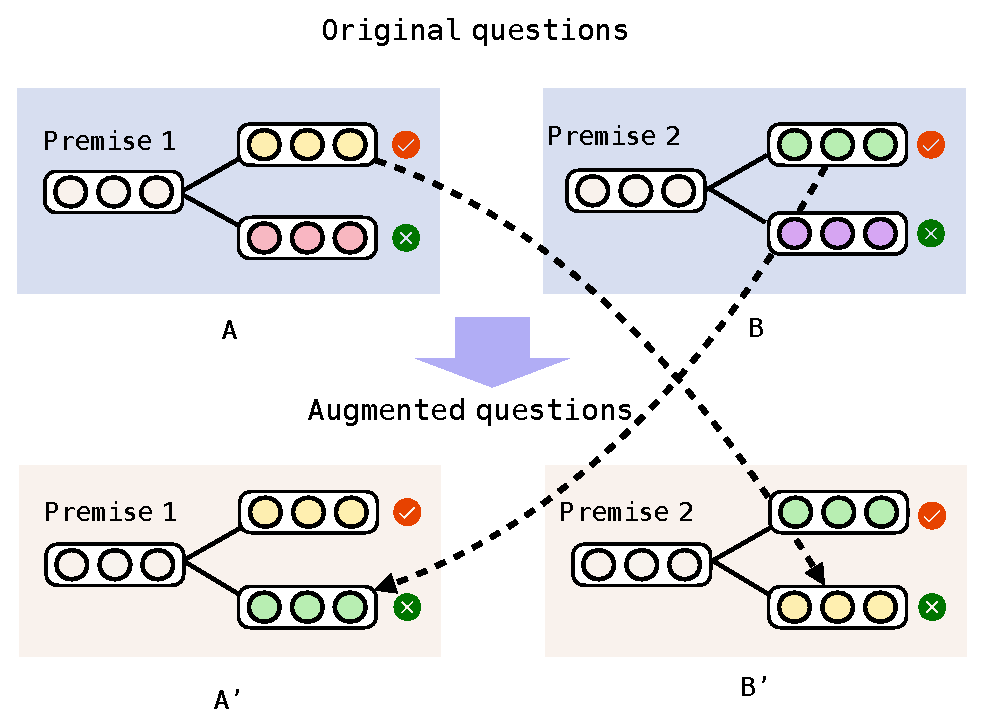
\includegraphics[width=\columnwidth]{figure/cross.eps}
 	\caption{The Crossover Operation: the true choice of both questions
 		are used to replace the false choices of these questions to create
 		two new proxy questions.}
 	\label{fig:cross}
 \end{figure}

In particular, for crossover operator, we only consider swapping the right choices between two questions 
rather than wrong choices. If we swapped the wrong choices, we could 
still produce two legitimate new questions. But these new questions can't
test short circuit, because: a) if a model
short-circuits on the right choice of question B (as in \figref{fig:cross}), 
swapping the wrong choice of B into question A doesn't make A' a good test, 
since the model is not sensitive to wrong choice; 
b) if a model short-circuits on the wrong choice of
question B, swapping the wrong choice of B into A will make A' 
easier to solve by the model, so it will 
still pick the right choice and pass the test.


%\begin{example}\label{ex:crossover}
%	\begin{description}
%		\item[Context:] The student knew the answer to the question.
%		\item[Choice 1:] He raised his hand . \Checkmark
%		\item[Original Choice 2:] He goofed off .\XSolidBrush
%		\item[Crossed Choice 2:] Dust got into his eyes.\XSolidBrush
%	\end{description}
%\end{example}

Compared with all other operations in class 1 and 2, 
crossover gives a proxy question that is most different from the original one,
but easier from human's perspective, because now the two choices maybe
quite unrelated. If the proxy question is not done correctly by the model, 
it's more indicative of a short circuit. So potentially, crossover
is a better short circuit test than others. 


Another advantage of crossover is that we can generate many wrong choices 
for an original question at a low cost, thus we can test each original question
more thoroughly. Whereas most other operations cannot produce 
variants of the original choice in large quantity. 
%The test cases for the third part is easy to construct, like mutation and voice~\cite{wsp2020acl}. 
%However, this type of testing is not sufficient to assess 
%whether the model has reasoning capabilities, 
%because solving these new cases does not require understanding of the previous premise. 
%We can't say for sure which of the reasons for the failure of 
%a specific case, 
%but it still reflects whether the model is robust or not. 

\subsection{Improving Model Robustness by Data Augmentation}
\label{sec:aug}
If a model is shown to short-circuit by the proxy tests, 
its performance may decline, especially when applied to out-of-domain test data.
%We make an assumption that these models are 
%limited by dataset and learned short circuits to make decision. 
To make models more robust, one natural thought is to generate more data to encourage models to focus on the 
relation between the premise and choices.
Intuitively, all the operations that can generate proxy tests
can be used to create more training data.
But in reality, most of these operations are not scalable and 
cannot generate enough data for training. 

The only two operations that do generate a lot of data
are crossover and its counterpart \textit{mutation}.
Besides the quantity, crossover is a good option for data augmentation,
because the two choices were originally true answers in their respective questions,
and presumably carry spurious features if the model was short-circuiting.
Hence to tell if one choice is better than the other, the model is forced to
consider the premise.
%We can also teach them to discover semantic and syntax problems with the advantage of the choice question format. 
%\KZ{Crossover not only can be used to test for
%short circuit, it can also be used to improve the model
%robustness. How to?}
%Both methods actually have the potential to teach the model 
%to consider the previous premise. First of all,  crossover is a replacement for the ``True'' choices, 
%models can not get the correct answer from the choices alone. 
%\KZ{The crossver operation inspired us to try mutation.}
Mutation operation swaps two consecutive words either in the right choice or wrong choice of the original MCQ, each with 50\% probability.
%Compared to crossover, 
Intuitively, mutation has the potential to be 
effective at improving model robustness:
it not only forces the model to look into the premise due to its
two very similar choices (same set of tokens), 
but also makes the model more
sensitive to find differences in word orders and 
enhances the model's prior grammatical knowledge. 
%Discuss the pros and cons of the two.
%Explain why mutation may not be a good choice for detecting
%short-circuit.

